\graphicspath{ {Implementation/Images/} }


\chapter{Validation}
\label{cha:implementation}

\section{Introduction}
In this chapter 

DiseaseMapping (generalization)
OSIM
Clusters
TensorFlow
DL4J

MENTION THAT LSTM CAN ALSO BE USED TO VALIDATE AND IS A BETTER WAY TO VALIDATE THIS METHOD


\section{Dataset}

To validate the approaches mentioned in chapter \ref{cha:background}, we used a dataset generated by Observational Medical Dataset Simulator Generation 2 (OSIM2) \cite{OSIM:online}. This dataset is used by Observational Medical Outcomes Partnership (OMOP) to validate their methods to predict the effects of drug treatments. It contains around $10$ million of hypothetical patients based on Thomson Reuters MarketScan Lab Database (MSLR). MSLR contains administrative claims between 2003 ad 2009 from a privately-insured population. \\

The OSIM2 dataset is contains multiple database tables which are dumped as comma-separated values (csv) files. To make it easier to work with this dataset, we joined the multiple files into one file with on each row an event of a patient containing all relevant information. The relevant information which is kept is: birth year, gender, condition type, condition, time difference since previous diagnosis, and season (summer, fall, winter, spring). Thus, one EHR is $7$ dimensional. \\	

Using our approaches on this dataset, we can compare our results to the found clusters in Anders Boeck Jensen et. \cite{Brunak:article}. Although these found clusters are not a golden standard, it is a first validation point for our approaches.


\section{Software}

\subsection{TensorFlow}

TensorFlow is an open-source machine learning software library released at the end of 2015 \cite{tensorflow:article}. It is developed by the Google Brain Team. \\
It provides a Python interface for efficient C++ code. After some time, we found that Tensorflow is not well documented at the moment and does not gave the needed freedom to easily rewrite some core features of their Word2Vec implementation, for example manipulating the internal trained lookup table.


\subsection{DeepLearning4Java}

DeepLearning4Java (DL4J) is an open-source machine learning software library released by Skymind \cite{dl4j:article}. \\
It runs on their scientific computing engine ND4J which provides fast matrix operations. DL4J is completely written in Java and provides a lot of freedom to manipulate lookup tables and extend their Word2Vec methods to work on abstract object like vectors. The developers are active on Gitter and offer a lot of information on how to use certain parts of DL4J. 


\section{Experiment Setup}

\subsection{Generalization}

As described in chapter \ref{cha:background}, we use generalized Word2Vec approaches to find patterns in EHR data. We use the OSIM dataset and represent each EHR as a $7$ dimensional vector. This vector is comparable to a word in a normal Word2Vec approach and functions as the abstract object in our generalized Word2Vec approaches. \\

Because we are working with high dimensional data, most instances of OMOP are quite unique. This is mainly due to a combination of specific disease codes and time intervals. To find patterns which are more general applicable, we start with generalizing our data. With generalizing we mean that values for some attributes are projected into categories. For example, the time intervals are projected into $4$ categories. \\

It is easy to generalize concepts as time intervals and demographics, for example we can say that people between the age $0$ and $10$ belong to category A. This becomes complex for disease diagnoses as it is domain specific and requires a lot of knowledge to generalize those. We talk about our solution to this in section \ref{sec:mapping}. \\

To see the effect of our generalization, see table \ref{tab:general}. You can see the $3$ most common vectors from our dataset before and after the generalization. \\

\begin{table}[!htb]
\centering

\label{tab:general}
\begin{tabular}{ll}
\cline{1-1}
\multicolumn{1}{|l|}{\textbf{Before Generalization}}                     & {\ul }                                   \\ \hline
\multicolumn{1}{|l|}{\textit{Vector}}                                    & \multicolumn{1}{l|}{\textit{Occurences}} \\ \hline
\multicolumn{1}{|l|}{{[}1956.0, 8532.0, 65.0, 5.00000701E8, 0.0, 3.0{]}} & \multicolumn{1}{l|}{17574}               \\ \hline
\multicolumn{1}{|l|}{{[}1954.0, 8532.0, 65.0, 5.00000701E8, 0.0, 3.0{]}} & \multicolumn{1}{l|}{17536}               \\ \hline
\multicolumn{1}{|l|}{{[}1955.0, 8532.0, 65.0, 5.00000701E8, 0.0, 3.0{]}} & \multicolumn{1}{l|}{17476}               \\ \hline
                                                                         &                                          \\ \cline{1-1}
\multicolumn{1}{|l|}{\textbf{After Generalization}}                      &                                          \\ \hline
\multicolumn{1}{|l|}{\textit{Vector}}                                    & \multicolumn{1}{l|}{\textit{Occurences}} \\ \hline
\multicolumn{1}{|l|}{{[}6.0, 8532.0, 65.0, 784955.0, 1.0, 3.0{]}}        & \multicolumn{1}{l|}{282086}              \\ \hline
\multicolumn{1}{|l|}{{[}7.0, 8532.0, 65.0, 784955.0, 1.0, 3.0{]}}        & \multicolumn{1}{l|}{235459}              \\ \hline
\multicolumn{1}{|l|}{{[}5.0, 8532.0, 65.0, 784955.0, 1.0, 3.0{]}}        & \multicolumn{1}{l|}{230216}              \\ \hline
\end{tabular}

\caption{Three most common vectors in our dataset before and after generalization}
\end{table}


\subsection{Disease Code Mapping}
\label{sec:mapping}

In the section we discuss the method to generalize the disease codes used to label the diagnoses in the OMOP dataset. The basic idea is that we want to generalize the diagnoses. For example, a bruise on your right leg is the same diagnoses as a bruise on your left leg. We would have liked to use the method described in \cite{icd10Mapping:article} to map the codes but therefore the mapping made by UMLS between ICD 10 and MedDRA is needed. This is however not publicly available. \\

The OMOP dataset uses MedDRA disease codes for the diagnoses. We described the MedDRA disease codes in chapter \ref{cha:context}. We mentioned that MedDRA does not have a clear hierarchy. With a clear hierarchy, it would be trivial to generalize a disease code to its highest hierarchy. \\
To solve this, we map the MedDRA disease codes to the ICD 10 disease codes. The reason behind this is that ICD 10 provides a clear and easy to use hierarchy. Besides the easy to use hierarchy, we also need the ICD 10 disease codes to make it possible to compare our results with Anders Boeck Jensen et. \cite{Brunak:article} as their results also use ICD 10 disease codes. \\

The mapping is based on the description of each disease code. Both MedDRA and ICD 10 have a short medical description of each code. Each description is first filtered from stop words. Afterwards, the MedDRA code is matched to the ICD 10 code based on the matching of both description. The matching is done on the highest percentage of words matching. \\

In figure \ref{fig:mappingStats}, we show the statistics of this mapping process. Note that we only take disease codes into account if they are also part of the OMOP dataset. In the figure, each bar represents the percentage of the words matching between descriptions. The height of the bars represent the percentage of all disease codes in the OMOP dataset who have this amount of matching percentage. \\

\begin{figure}[!htb]
	\centering
	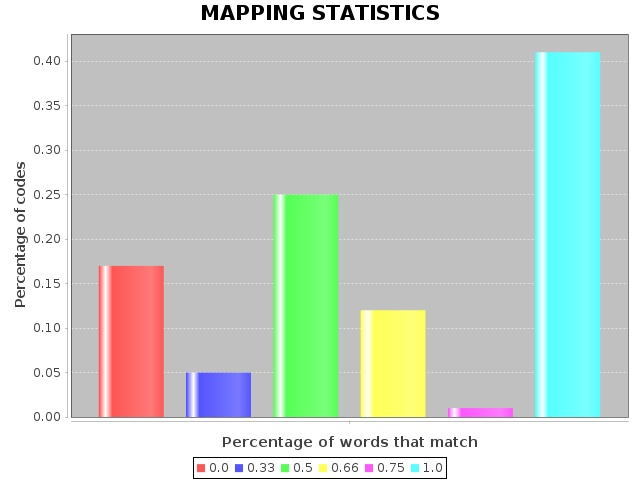
\includegraphics[width=0.7\textwidth]{mappingStats.jpeg}
	\caption{Statistics of the mapping approach}
	\label{fig:mappingStats}
\end{figure}

We have an average of $63$ \% of the words from the description that matches between MedDRA and ICD 10 descriptions. We also see that around $85$ \% of all the disease code mappings have a match of atleast $33$ \%. We assume this is already a good mapping as medical terms are quite specific and if $33$ \% matches, the upper hierarchy will be a good enough match. For the codes which have a zero percent match, the Damerau-Levenshtein algorithm \cite{edit:article} is applied. The algorithm calculates the edit distance between two strings using character insertion, character deletion, character replacement, and adjacent character swaps. The description with the lowest edit distance, is then chosen as best match. \\
Another option would have been to remove those codes from our dataset. As an EHR contains more information than only the disease code, a lot of other information would have been lost. This however is not tested and is a possibility for future work. \\

\section{Results}

\subsection{Experiments}

To test our approaches we will compare our results with the clusters found from Anders Boeck Jensen et. \cite{Brunak:article}. For this, we also need to generate our own found clusters. This method is described in this section. Note that the comparison with the Danish paper is not ideal but it is currently the largest study performed on EHRs. We refer to chapter \ref{cha:futureWork} for more information about another possible experiment in the future. \\

First we apply our approaches on the OSIM dataset. For a description of the used parameters and their functions, see section \ref{sec:parameters}. As end result, we get a lookup table containing the mapping between the old vector space and the new one. From this lookup table, we take EHRs and find their k-nearest neighbors depending on their mapping in the new vector space (see section \ref{sec:parameters} for more information about clusterK). Depending on the approach, we take certain EHRs. For the generalized Word2Vec, we check all EHRs in the lookup table. For the knn Word2Vec, we only check the complete new instances added to the lookup table using the knn method. For DeepWalk, we again take all EHRs in the lookup table. \\

Based on the formed clusters from our lookup table (Word2Vec clusters), we can now compare it to the Danish clusters. We test the matching between the two clusters based on two experiments. \\
The first one is as follows:

\begin{itemize}

\item We start with an element $e_{wv}$ from the lookup table and form a Word2Vec cluster $C_{wv}$ around it.
\item We then check to which Danish cluster $C_d$ element $e_{wv}$ belongs.
\item For each element in $C_{wv}$, we check if it belongs to $C_d$.
\begin{itemize}
\item If it does, we add $1$ to the number $t_{matches}$.
\item If it does not, we add $1$ to the number $t_{non\_matches}$.
\end{itemize}
\item After doing this for all elements in $C_{wv}$, we calculate the match percentage as $p_{match} = \frac{t\_{matches}}{t_{matches} + t_{non\_matches}}$.

\end{itemize}

The second one is as follows:

\begin{itemize}

\item We start with an element $e_{wv}$ from the lookup table and form a Word2Vec cluster $C_{wv}$ around it.
\item We then check to which Danish cluster $C_d$ element $e_{wv}$ belongs.
\item We set $t_{d}$ equals to the amount of elements in $C_d$.
\item For each element in $C_{wv}$, we check if it belongs to $C_d$.
\begin{itemize}
\item If it does, we add $1$ to the number $t_{matches}$.
\end{itemize}
\item After doing this for all elements in $C_{wv}$, we calculate the match percentage as $p_{match} = \frac{t\_{matches}}{t_{d}}$.

\end{itemize}

For each method, we calculate the average $p_{match}$ over all elements of the lookup table and keep track of the maximum and minimum value for $p_{match}$.


\subsection{Parameters}
\label{sec:parameters}

The effectiveness of a neural network like the one used to learn the disease embeddings, depends on parameter tuning \cite{tuning:article}. Therefore we explored some different settings. Note that this is not an extensive parameter tuning setup, but an overview on the effect and logic behind some parameters. An extensive parameter tuning setup is possible as future work. \\

In table \ref{tab:parameters}, you can see an overview of the different parameters for each approach. For each approach, all possible combinations of the mentioned parameters have been tested. \\

\begin{table}[!htb]
\centering

\label{tab:parameters}
\begin{tabular}{llll}
\hline
Parameter                                    & Generalized Word2Vec  & Knn Word2Vec          & DeepWalk              \\ \hline
\multicolumn{1}{l|}{Vectorlength}            & {[}50, 100{]}         & {[}50, 100{]}         & {[}50, 100{]}         \\
\multicolumn{1}{l|}{Batch Size}              & 500                   & 500                   & 500                   \\
\multicolumn{1}{l|}{Epoch}                   & 1                     & 1                     & 1                     \\
\multicolumn{1}{l|}{Window Size}             & {[}5, 10, 15{]}       & {[}5, 10, 15{]}       & {[}5, 10, 15{]}       \\
\multicolumn{1}{l|}{Learning Rate}           & {[}0.025, 0.1{]}      & {[}0.025, 0.1{]}      & {[}0.025, 0.1{]}      \\
\multicolumn{1}{l|}{Minimum Word Frequency} & {[}5, 10{]}           & {[}5, 10{]}           & {[}5, 10{]}           \\
\multicolumn{1}{l|}{ClusterK}                & {[}100, 1000, 5000{]} & {[}100, 1000, 5000{]} & {[}100, 1000, 5000{]} \\
\multicolumn{1}{l|}{K}                       & /                     & {[}10, 50, 100{]}     & /                     \\
\multicolumn{1}{l|}{Walklength}              & /                     & /                     & {[}5, 10, 15{]}      
\end{tabular}

\caption{Parameters which are tested for the different approaches}
\end{table}

\noindent\textbf{Vectorlength} decides the dimensions of the new vector space to which the diseases are projected to. A larger size is more expressive but a smaller size decreases the complexity of the vocabulary after the training. Each dimension can be seen as a representation of an unknown linear relation to some context-disease pairs \cite{vl:article}. \\
\textbf{Batch size} is the number of training examples used in one gradient descent step (both forward and backward pass). \\
\textbf{Epoch} is the amount of times you go over all the training examples and use them to train your neural network. \\
\textbf{Window size} is the size of the n-gram we use to create contexts. A larger window tends to make more specific contexts and therefore get a better model \cite{w2vOriginal:article} \cite{windowSize:article}. \\
\textbf{Learning rate} decides how the weights are adjusted during backpropagation. A large value can make the neural network learn faster but may also cause the network to not learn at all. A small value on the other hand can cause a slow convergence or overfitting \cite{lr:article}. Note that in our implementation there is a decay of the learning rate as the number of examples left decreases. \\
\textbf{Minimum Word Frequency} removes instances from the training set below the minimum. A low frequency causes some instances to only have a few contexts where relations can be learned from. So a higher frequency could improve the accuracy for a Word2Vec model but also throw away information. Note that the influence of this parameter is not well researched. \\
\textbf{ClusterK} is the parameter which creates the Word2Vecclusters as described in the previous section. A higher clusterK causes the Word2Vec cluster to be larger and a lower value the other way around. \\
\textbf{K} is a specific parameter for the knn Word2Vec approach. It decides on how many nearest neighbors the new vector representation is based on. For more explanation see chapter \ref{cha:background}. \\
\textbf{Walklength} is a specific parameter for DeepWalk. It decides how long the generated sequence will be. For more explanation see chapter \ref{cha:background}. \\


\subsection{Generalized Word2Vec}
Dataset percentage

\subsubsection*{ClusterK}

\subsubsection*{ClusterK}

\subsubsection*{ClusterK}

\subsection{K-Nearest Neighbors Word2Vec}

\subsection{DeepWalk}



\section{Conclusion}





%%% Local Variables: 
%%% mode: latex
%%% TeX-master: "thesis"
%%% End: 
